{\let\cleardoublepage\relax \chapter{Wstęp}}
\label{cha:wstep}

Tematem pracy inżynierskiej jest opracowanie aplikacji internetowej do nauki języków obcych

\section{Cel Aplikacji}

Zadaniem aplikacji jest umożliwienie nauki wybranych słówek danego języka obcego z pomocą wirtualnych fiszek, które będą prezentowane użytkownikowi w nieregularnych odstępach czasowych obliczanych na podstawie poprawności udzielonych odpowiedzi.



Coraz większą popularność w dzisiejszym świecie zdobywają aplikację internetowe. Ich niewątpliwą zaletą jest możliwość uruchomienia ich na dowolnym urządzeniu posiadającym internet i przeglądarkę internetową. Jeszcze do nie dawna były to jedynie komputery i urządzenia mobilne, lecz wraz ze wzrostem popularności inteligentnych technologii (po ang. smart) coraz więcej produktów codziennego użytku potrafi łączyć się z internetem. Do takich urządzeń zaliczają się mikrofalówki, lodówki, telewizory i wiele innych.

\begin{figure}[h]
	\centering
	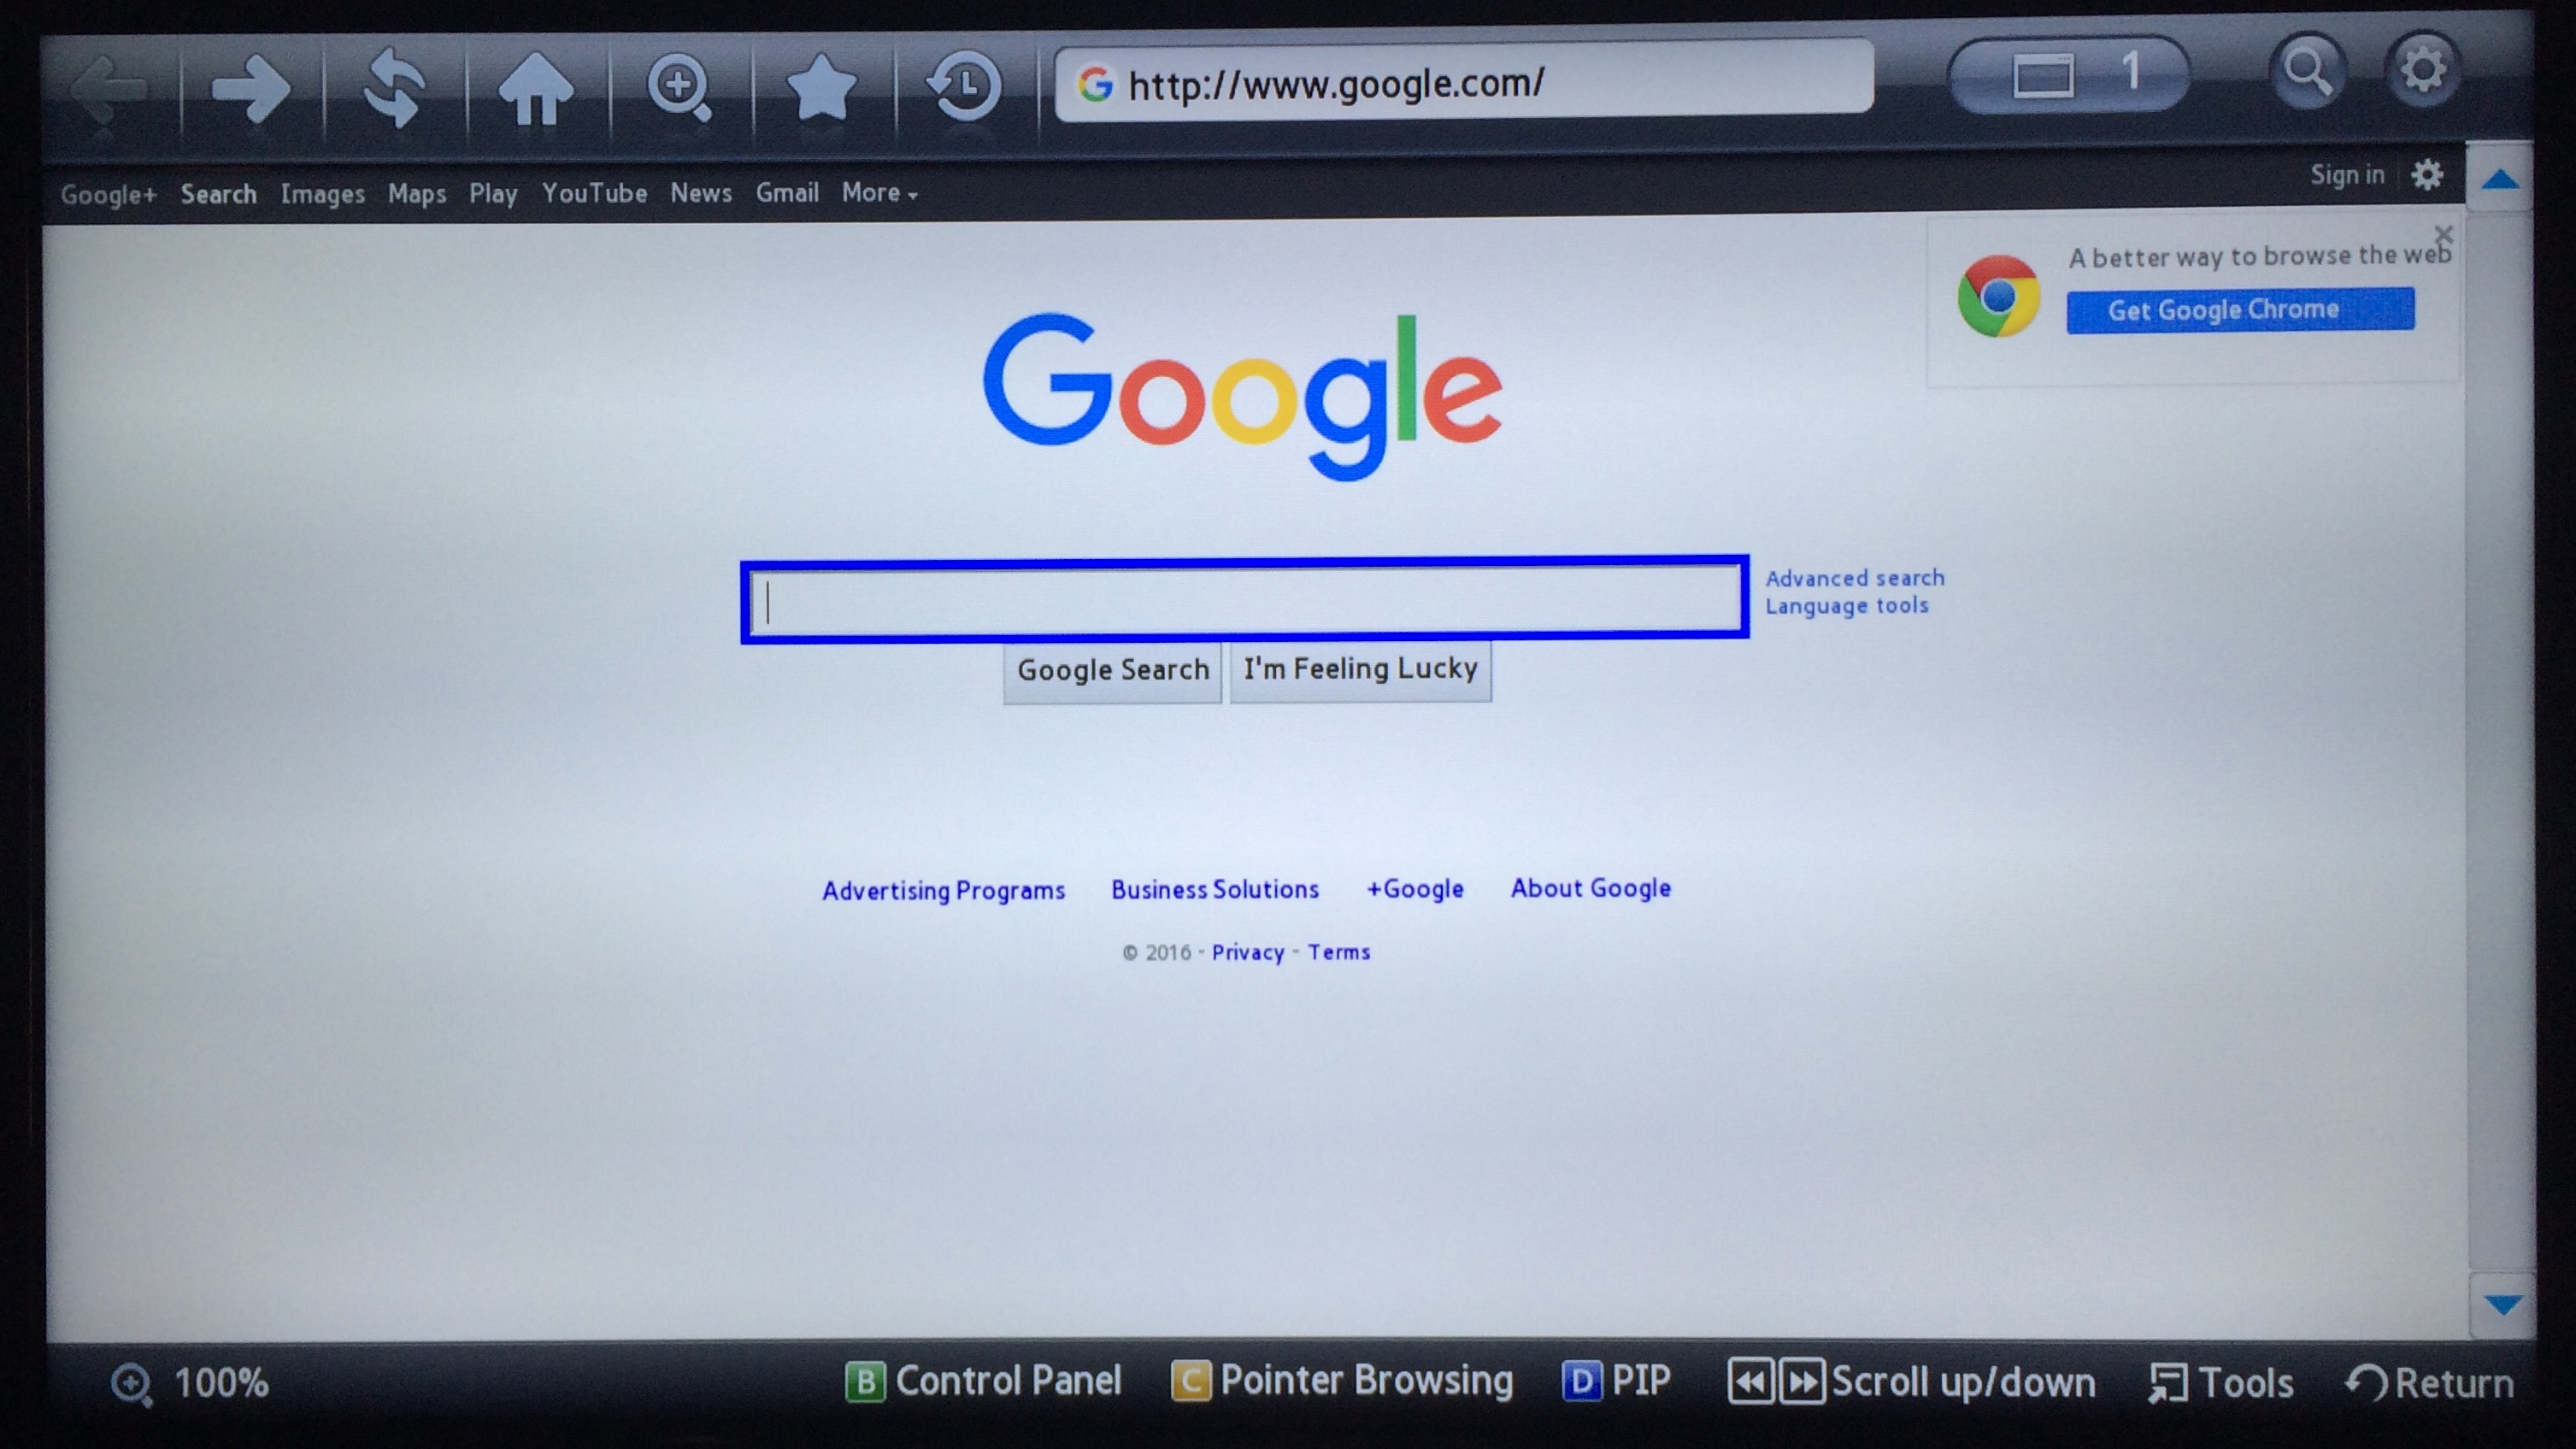
\includegraphics[height=50.5mm]{images/Browser.jpg}
	 \caption{Przeglądarka internetowa wbudowana w telewizor.}
\end{figure}




\newpage
{\let\cleardoublepage\relax \chapter{Założenia projektu}}
\subsection{Założenia aplikacji}

Zadaniem aplikacji jest umożliwienie nauki wybranych słówek danego języka obcego z pomocą wirtualnych fiszek, które będą prezentowane użytkownikowi w nieregularnych odstępach czasowych obliczanych na podstawie poprawności udzielonych odpowiedzi.
Program powinien umożliwiać:
\begin{itemize}
	\item Dodawanie, modyfikowanie i usuwanie fiszek.
	\item 
\end{itemize}


Program został stworzony w języku C\# z użyciem frameworka ASP.NET MVC. Wszystkie dane są przechowywane na serwerze Microsoft SQL. Po stronie klienta użyto języka HTML wraz z arkuszami styli stworzonymi w oparciu o język SASS. Wszystkie skrypty napisano w języku Scala, który jest potem kompilowany przez narzędzie Scala.js do 